\section{Evaluation}

Using the settings in the implementation section, we measure 
end-to-end delay between an UE and different Internet servers. 
The delay inside the core network is the delay 
between VMs in a same physical machine. Although this 
delay is overly small (less than 10ms) and unrealistic, we argue that 
delay gain shown in this evaluation section is 
the worst case scenario (in other words, with real networks, we 
would expect a higher gain compared to what showing here).

\begin{figure}[hbtp]
\centering
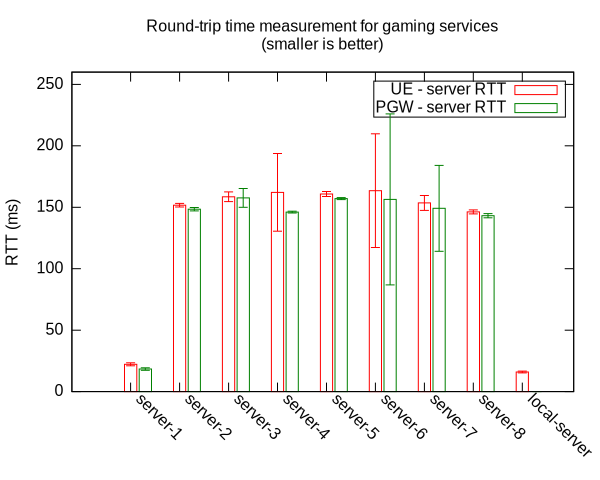
\includegraphics[scale=0.11]{./figure/game-server-rtt.png}
\caption{Game service RTT}
\label{fig:game-rtt}
\end{figure}

We pick 5 most popular streaming services based on ~\cite{http://www.techsupportalert.com:2013} 
and top 10 Minecraft ~\cite{Minecraft.net:2013} online game servers based on ~\cite{http://www.serverpact.com:2013} 
to measure end-to-end round-trip times (RTTs) between an UE/PGW and the servers. A round-trip time is 
measured using 50 ICMP pings and the average delay is shown. 
In 5 streaming services, one does not allow ICMP ping. Two listed game servers are
also dead.

\begin{figure}[hbtp]
\centering
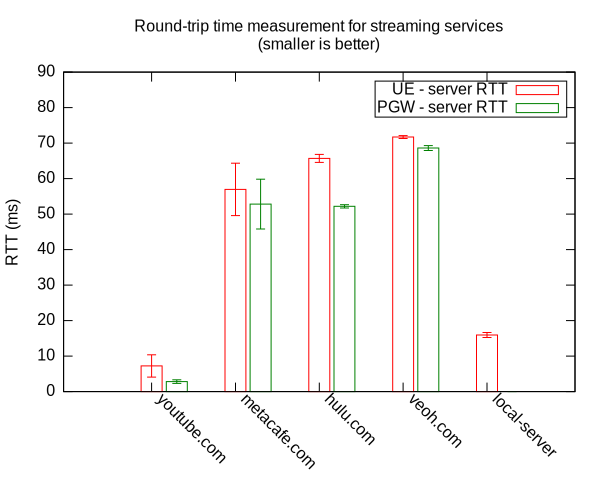
\includegraphics[scale=0.11]{./figure/streaming-server-rtt.png}
\caption{Stream services RTT}
\label{fig:stream-rtt}
\end{figure}

Compared to contacting servers in the Internet, using the offloading server 
significantly reduces the RTT as in figure ~\ref{fig:game-rtt} and 
~\ref{fig:stream-rtt} (offloading RTT is about 18ms while accessing
Internet servers would result in about 4 times higher delay for streaming services and 
about 9 times higher delay for gaming services). Green boxes show RTTs between the PGW and 
Internet servers (these are essentially Internet delays), the red boxes show the RTTs between 
the UE and the server (total end-to-end delay). Surprisingly, offloading does not defeat 
youtube.com. This could be speculated as: (1) heavy processing 
at the controller (since we intercept \textit{every} packet) adds extra delay to the path, (2) youtube.com 
might deploy CDN servers very closed to the PGW so that the Internet delay is small, (3) since the core delay is 
so small, this eliminates the gain of offloading approach over hierarchical routing issue and in the mean time this 
eliminates the delay that youtube.com should have in reality.



